\documentclass[journal]{IEEEtran}
\usepackage{graphicx} % Required for inserting images
\usepackage{amsmath} % For \text in math mode
\usepackage{float}
\usepackage{hyperref}
\usepackage{algorithm}
\usepackage{algpseudocode}
\usepackage{amssymb}
\usepackage{booktabs}
\usepackage{siunitx}
\usepackage{tikz}
\usepackage{adjustbox}
\usepackage{multirow}


\usepackage{cleveref}
\crefname{section}{Section}{Sections}
% \crefname{subsection}{Subsection}{Subsections}

\usetikzlibrary{arrows.meta,positioning}

\title{}
\date{}  % This hides the date
\author{}  % Optional: hides the author if you don’t want one
\begin{document}

% \maketitle 

% \begin{abstract}

% \end{abstract}

% \begin{IEEEkeywords}

% \end{IEEEkeywords}


\section{Introduction}
\label{sec:introduction}

\subsection{Background}

Automatic speech recognition (ASR) has progressed significantly with deep sequence models. The Transformer architecture \cite{vaswani2017attention}
 and its convolution-augmented variant, the Conformer \cite{gulati2020conformer}, now achieve state-of-the-art accuracy on benchmarks such as LibriSpeech, outperforming recurrent and CNN models. Self-supervised pretraining \cite{baevski2020wav2vec} further boosts accuracy, and streaming architectures like the RNN-Transducer \cite{Graves2012SequenceTW}, and its Transformer-based extensions enable low-latency transcription. However, these systems are static: they use a fixed model for all inputs. In realistic deployments, acoustic conditions such as noise, channel and speaker can vary unpredictably over time. A static model may be suboptimal across domains or may waste capacity on easy inputs. A model that performs well under certain acoustic conditions may not generalize equally
 well to others, leading to fluctuations in transcription quality across inputs. This observation suggests that no single STT system can be expected to perform optimally across all scenarios. Instead,
different models often demonstrate strengths  in different regimes, forming a collection of complementary experts. Using this
diversity requires mechanisms that can adaptively determine
which model is most suitable for a given input, rather than
committing to a fixed system. Such adaptive strategies aim to
retain the efficiency of single-model inference while benefiting
from the diversity of multiple pretrained systems.

A key difficulty in this setting is predicting the performance of candidate models without explicitly executing them. Observable properties of the audio signal, such as acoustic
statistics, temporal dynamics, and learned representations,
provide useful cues for this purpose. Nevertheless, many
existing approaches treat each audio segment as an independent
unit, making selection decisions based solely on local
information. This ignores an important aspect of speech: its
inherently sequential nature.

In practical scenarios such as conversations, meetings, or
continuous recordings, audio segments are temporally
correlated. Consecutive segments often share common attributes,
including speaker identity, background conditions, and channel
characteristics. Furthermore, transitions between different
acoustic regimes typically occur gradually rather than
instantaneously. As a result, the suitability of a particular
STT model at a given time step is influenced not only by the
current segment, but also by its surrounding context.

Neglecting these temporal relationships can lead to unstable
or suboptimal selection behavior, particularly in long-form
audio where conditions evolve over time. This motivates the
development of adaptive STT frameworks that explicitly model
sequential dependencies and incorporate contextual information
into the selection process. In this work, we explore this
direction by formulating STT model selection as a sequential
decision problem and introducing a context-aware routing
framework that leverages temporal structure to improve
selection accuracy.
 
 %By contrast, dynamic architectures such as sparsely-gated Mixture-of-Experts (MoE) networks can adaptively allocate capacity per input \cite{you2021speechmoe,fedus2021switch}. For example, GShard showed that conditional computation can scale Transformers to hundreds of billions of parameters without raising per-token cost
 %and the Switch Transformer simplifies MoE routing to train trillion-parameter models efficiently In speech, dynamic routers have been explored: the SpeechMoE family
 %dispatches frames to expert sub-networks using a shared embedding, and a recent Streaming Conformer-MoE reduced WER by ~12\% while halving active parameters


%Building on these ideas, we introduce a sequential STT router that operates at the level of audio segments rather than individual frames or tokens. In essence, given a long audio stream split into segments (by silence or fixed windows), the router observes embeddings of each segment (which may come from an ASR encoder or acoustic front-end) and selects the most appropriate ASR expert for that segment. A Transformer-based routing function uses self-attention over a sliding window of recent segments, capturing context such as speaker continuity or acoustic drift, to produce expert preference scores. At inference time, only the selected ASR expert is invoked for each segment so latency remains that of one model per segment  while the router adds minimal compute.

\subsection{Related Work}
\label{sec:related_work}

Modern end-to-end ASR often uses attention-based encoder-decoder or transducer models. The original Transformer eliminated recurrence in sequence-to-sequence tasks and has been widely adapted for speech. In ASR, the Conformer architecture
augments self-attention with convolutional modules to better model local speech structure; it achieved near-state-of-the-art LibriSpeech WERs (2.1% clean/4.3% other) while remaining compact
. Self-supervised pretraining (e.g. wav2vec 2.0
) learns useful speech representations, allowing models to reach very low error rates with limited labels. Streaming extensions include the RNN-Transducer
 and Transformer-Transducer models (which combine attention with transducer output), as well as chunk-based Conformers for real-time use. These models focus on accuracy and (for streaming ones) low latency, but remain static in that all inputs use the same network.

Streaming ASR places strict latency constraints. RNN-T was a seminal approach for on-the-fly ASR with fixed delay. Recent efforts apply Transformer/Conformer backbones to streaming by attention truncation or recurrence (e.g. Emformer, Streaming Transformer-Transducer) to meet real-time budgets. These approaches optimize architecture to reduce delay but do not adapt computation per input. In contrast, our router is inherently sequential and can be used in a streaming pipeline: at each segment boundary it uses contextual info to pick a model, then immediately invokes that expert (with only its output carrying the latency cost). Thus latency stays low (one model’s inference), while adaptation occurs invisibly in parallel.

Routing and Mixture-of-Experts: Our work is inspired by sparse MoE and conditional computation. Early Mixture-of-Experts (Shazeer et al. 2017) enabled enormous capacity by routing tokens to only one expert subnetwork
. This idea was massively scaled in Google’s GShard (2020) and Follow-up Switch Transformer (2021)
: models with hundreds of billions of parameters were trained with sparsely-gated MoE layers at constant cost. GShard demonstrated a 600B-parameter translation model using dynamic routing
, while Switch simplified the routing algorithm for efficiency
. Beyond NLP, MoE has been applied in vision and other domains as well. All these models perform intra-network routing: each input token or frame is dispatched to expert feedforward layers or networks. By contrast, our router performs inter-model routing: it selects among whole ASR models (or large subnetworks) at each segment. This yields coarse-grained conditional computation: we trade finer token-level routing for more efficient segment-level decisions.

There is growing work on adaptive or multi-domain ASR. You et al. (2021) proposed SpeechMoE, adding MoE layers to a CTC model with a learned embedding for the router
. SpeechMoE achieved substantial CER reductions (7–23% relative) over a static model
 by dynamically routing frames to experts. A follow-up SpeechMoE2 (2022) improved routing by feeding domain- and accent-embeddings to the router
. More recently, Hu et al. (2023) introduced a Switch-Conformer MoE: a multilingual streaming Conformer with MoE FFN layers. They report an 11.9% relative WER drop over a baseline, activating only 53% of parameters during inference
. Our router differs from these in granularity and scope: whereas SpeechMoE layers route individual frames within a model, our router chooses an entire expert per segment. This yields lower overall switching frequency and allows specialization at the whole-model level.

Conditional Computation and Routing: More broadly, conditional computation in neural networks includes techniques like dynamic skipping of layers (e.g. Skip-RNN, BlockDrop), early-exit classifiers, or adaptive layers. For sequence models, some work (e.g. Routing Transformer
) learns sparse attention patterns via content-based routing, reducing complexity from quadratic to sub-quadratic. Roy et al.’s Routing Transformer routes queries to a subset of keys using a k-means router, achieving state-of-the-art language modeling on long contexts
. This is complementary to our goal: they reduce attention cost, while we route between entire subnetworks. Other NLP works (e.g. BASELayers
) explore sparse capacity allocation for multi-task learning, highlighting issues like expert specialization and training stability. In our speech context, we assume expert models are pre-trained on diverse data, and focus the router’s learning on choosing among them. The main trade-off is between granularity and overhead: our segment-level router has fewer switching decisions (favoring stability and efficiency) but may be less responsive to rapid changes than frame-level gating. We mitigate this with temporal context and cost-sensitive loss.

% A large body of research has focused on improving the robustness of
% automatic speech recognition systems under diverse acoustic conditions,
% including noise, reverberation, channel variability, and speaker
% heterogeneity. Approaches such as multi-condition training,
% data augmentation strategies, and domain adaptation techniques aim to
% expose models to a wide range of acoustic scenarios during training,
% thereby improving generalization at inference time.
% More recently, self-supervised learning methods and large-scale
% pretrained speech encoders have significantly enhanced representation
% quality, enabling models to perform well across previously unseen
% conditions. These methods primarily pursue a single-model paradigm,
% where robustness is achieved by increasing model capacity and training
% data diversity. In contrast, our work considers a complementary
% perspective: instead of improving a single model, we exploit a pool of
% pretrained STT systems and focus on selecting the most suitable model
% for each input.

% Another line of work aims to leverage multiple ASR systems through
% ensemble and system combination techniques. Classical approaches such
% as hypothesis alignment and voting schemes combine outputs from
% multiple decoders to reduce transcription errors. Extensions to these
% methods include confusion network construction, posterior-based
% fusion, and minimum Bayes risk decoding, as well as more recent neural
% fusion techniques that aggregate intermediate or final predictions
% from multiple models. While such approaches often yield improvements
% in transcription accuracy, they require executing multiple STT models
% for each input and performing additional alignment or fusion steps,
% leading to increased computational cost and latency. In contrast,
% model selection frameworks aim to retain the benefits of model
% diversity while executing only a single expert at inference time,
% making them more suitable for large-scale or real-time deployments.

% Adaptive expert selection is also closely related to the broader
% literature on mixture-of-experts (MoE) and conditional computation.
% In classical MoE models, a gating network assigns input-dependent
% weights to multiple experts, and both the experts and the gating
% mechanism are trained jointly within a unified architecture.
% Recent developments in sparse and large-scale MoE systems further
% improve efficiency by activating only a subset of parameters for each
% input. However, these approaches typically assume that experts share
% a common backbone and are optimized end-to-end under a unified
% objective. In contrast, our setting considers independently pretrained
% STT systems as fixed experts, with no parameter sharing or joint
% training. The routing mechanism operates as a separate model that
% learns to predict expert suitability based on input characteristics,
% making it possible to incorporate heterogeneous models without
% modifying their internal architectures.

% A related direction explores confidence estimation and quality
% prediction for ASR outputs. Confidence scores derived from posterior
% probabilities or auxiliary prediction models have been used for
% hypothesis selection, rescoring, and fallback strategies. Similarly,
% domain classification and environment detection methods attempt to
% route inputs to specialized models based on coarse categorical
% attributes such as noise type or speech domain. While effective in
% certain scenarios, these approaches either require partial decoder
% execution to obtain confidence measures or rely on predefined domain
% boundaries that may not capture fine-grained variability in acoustic
% conditions. In contrast, feature-based selection methods aim to
% predict expert performance directly from input representations,
% enabling lightweight routing decisions without running multiple STT
% systems.

% Most existing adaptive selection approaches formulate the problem as
% an instance-wise decision task, where each audio segment is processed
% independently. This assumption neglects the temporal structure of
% speech signals, where consecutive segments are often correlated and
% share common acoustic characteristics. In long-form recordings, such
% as conversations and meetings, factors such as speaker identity,
% background noise, and channel conditions tend to persist over time or
% change gradually. Ignoring these temporal dependencies can limit the
% effectiveness of selection mechanisms, leading to unstable or
% suboptimal routing decisions. In this work, we address this limitation
% by modeling adaptive STT selection as a sequential decision problem
% and incorporating temporal context into the routing process, enabling
% more consistent and context-aware expert selection across audio
% streams.


\subsection{Contributions}

Our contributions are summarized as follows:

\begin{itemize}

\item We introduce a sequential adaptive STT routing framework that
extends instance-wise model selection to a sequence-aware setting,
where expert selection decisions are conditioned on the temporal
context of neighboring audio segments. This enables the system to
capture evolving acoustic conditions and improve selection reliability
in long-form speech.

\item We formulate adaptive STT model selection as a contextual
sequence decision problem and propose a transformer-based routing
function that maps sequences of segment-level feature representations
to expert preference distributions. The model leverages self-attention
to capture temporal dependencies such as speaker continuity,
environment persistence, and gradual acoustic drift.

\item We develop a cost-sensitive training objective based on expected
transcription error, which directly optimizes the routing model with
respect to task-level performance measures such as WER. The framework
naturally supports alternative error metrics, making it loss-agnostic
and adaptable to different evaluation criteria.

\item We incorporate temporal consistency into the routing process
through a context-aware formulation that promotes stable expert
selection across consecutive segments, reducing unnecessary switching
while preserving responsiveness to meaningful changes in acoustic
conditions.

\item Our framework performs input-adaptive STT model selection using a
lightweight routing mechanism operating on pre-extracted acoustic and
embedding-based features. The approach remains feature-agnostic and
compatible with arbitrary discriminative representations, while
introducing only minimal computational overhead beyond a single STT
model execution at inference time.

\item The proposed framework is routing-model agnostic and can be
instantiated using different sequence modeling architectures. While we
focus on transformer-based routing in this work, the formulation allows
for alternative temporal models such as recurrent or convolutional
sequence learners without modifying the overall framework.

\end{itemize}


\subsection{Organization}

The remainder of the paper is organized as follows.
\cref{sec:problem} formalizes the sequential adaptive STT selection
problem. \cref{sec:workdone} presents the proposed framework,
including the sequential feature representation, transformer-based
routing model, and training objective. \cref{sec:experiments}
describes the experimental setup and empirical evaluation.
Finally, \cref{sec:conclusion} concludes the paper.

\section{Problem Description}
\label{sec:problem}

We study adaptive speech-to-text (STT) transcription for temporally ordered audio streams composed of a large number of audio segments denoted by $\{x_t\}_{t=1}^{T}$, where $T$ is significantly large. In realistic speech recordings such as conversations, meetings, or long-form audio streams, the acoustic conditions and speaker characteristics evolve over time. Properties of each audio segment, including background noise level, speaker identity, accent, speaking rate, recording quality, and acoustic clarity, may vary gradually or abruptly across the sequence. Consequently, different state-of-the-art STT algorithms may exhibit varying levels of transcription performance depending on the acoustic conditions associated with each segment \cite{yu2016asrdeep,li2014overviewrobust}. Since these conditions change over time and are not known in advance, it is generally unknown which STT algorithm will perform best for each segment in the sequence.

Let $\mathcal{A} = \{A_1, A_2, \ldots, A_K\}$ denote a finite set of $K$ distinct STT algorithms, where $A_j \in \mathcal{A}$ represents the $j$-th algorithm. For each audio segment $x_t$, the transcription produced by the $j$-th STT algorithm is denoted by
\[
T_{t,j} = A_j(x_t).
\]
Each transcription $T_{t,j}$ can be evaluated using a transcription error measure defined with respect to the ground-truth transcription $R_t$ associated with segment $x_t$. Using standard evaluation metrics such as the Word Error Rate (WER) or other suitable transcription accuracy measures \cite{li2014overviewrobust}, we define the transcription loss incurred by using algorithm $A_j$ on segment $x_t$ as
\[
\ell(T_{t,j}, R_t),
\]
where $\ell(\cdot,\cdot)$ denotes the chosen error metric.

In practice, applying all $K$ STT algorithms to every incoming segment in order to select the best transcription is computationally expensive and inefficient. Instead, the goal is to select a single STT algorithm for each segment in a manner that minimizes the overall transcription error across the entire sequence. Let $j_t \in \{1,2,\ldots,K\}$ denote the index of the STT algorithm selected for segment $x_t$. The resulting transcription for that segment is therefore given by
\[
\hat{T}_t = A_{j_t}(x_t).
\]

The objective is to determine a sequence of algorithm selections $\{j_t\}_{t=1}^{T}$ that minimizes the cumulative transcription error over the entire audio stream:
\begin{center}
$\displaystyle
\sum_{t=1}^{T} \ell(T_{t,j_t}, R_t).
$
\end{center}

Unlike independent algorithm selection problems where each decision is made solely based on the current input, the performance of STT algorithms may exhibit temporal correlations across consecutive audio segments due to evolving acoustic environments, speaker continuity, or recording conditions. Therefore, selecting the most suitable algorithm for a given segment may benefit from considering information from neighboring segments within the sequence. In the following section, we introduce a framework that models this sequential algorithm selection problem and determines the STT algorithm for each segment while accounting for temporal dependencies across the audio stream.


\section{Workdone}
\label{sec:workdone}

% \begin{figure*}[t]
%     \centering
%     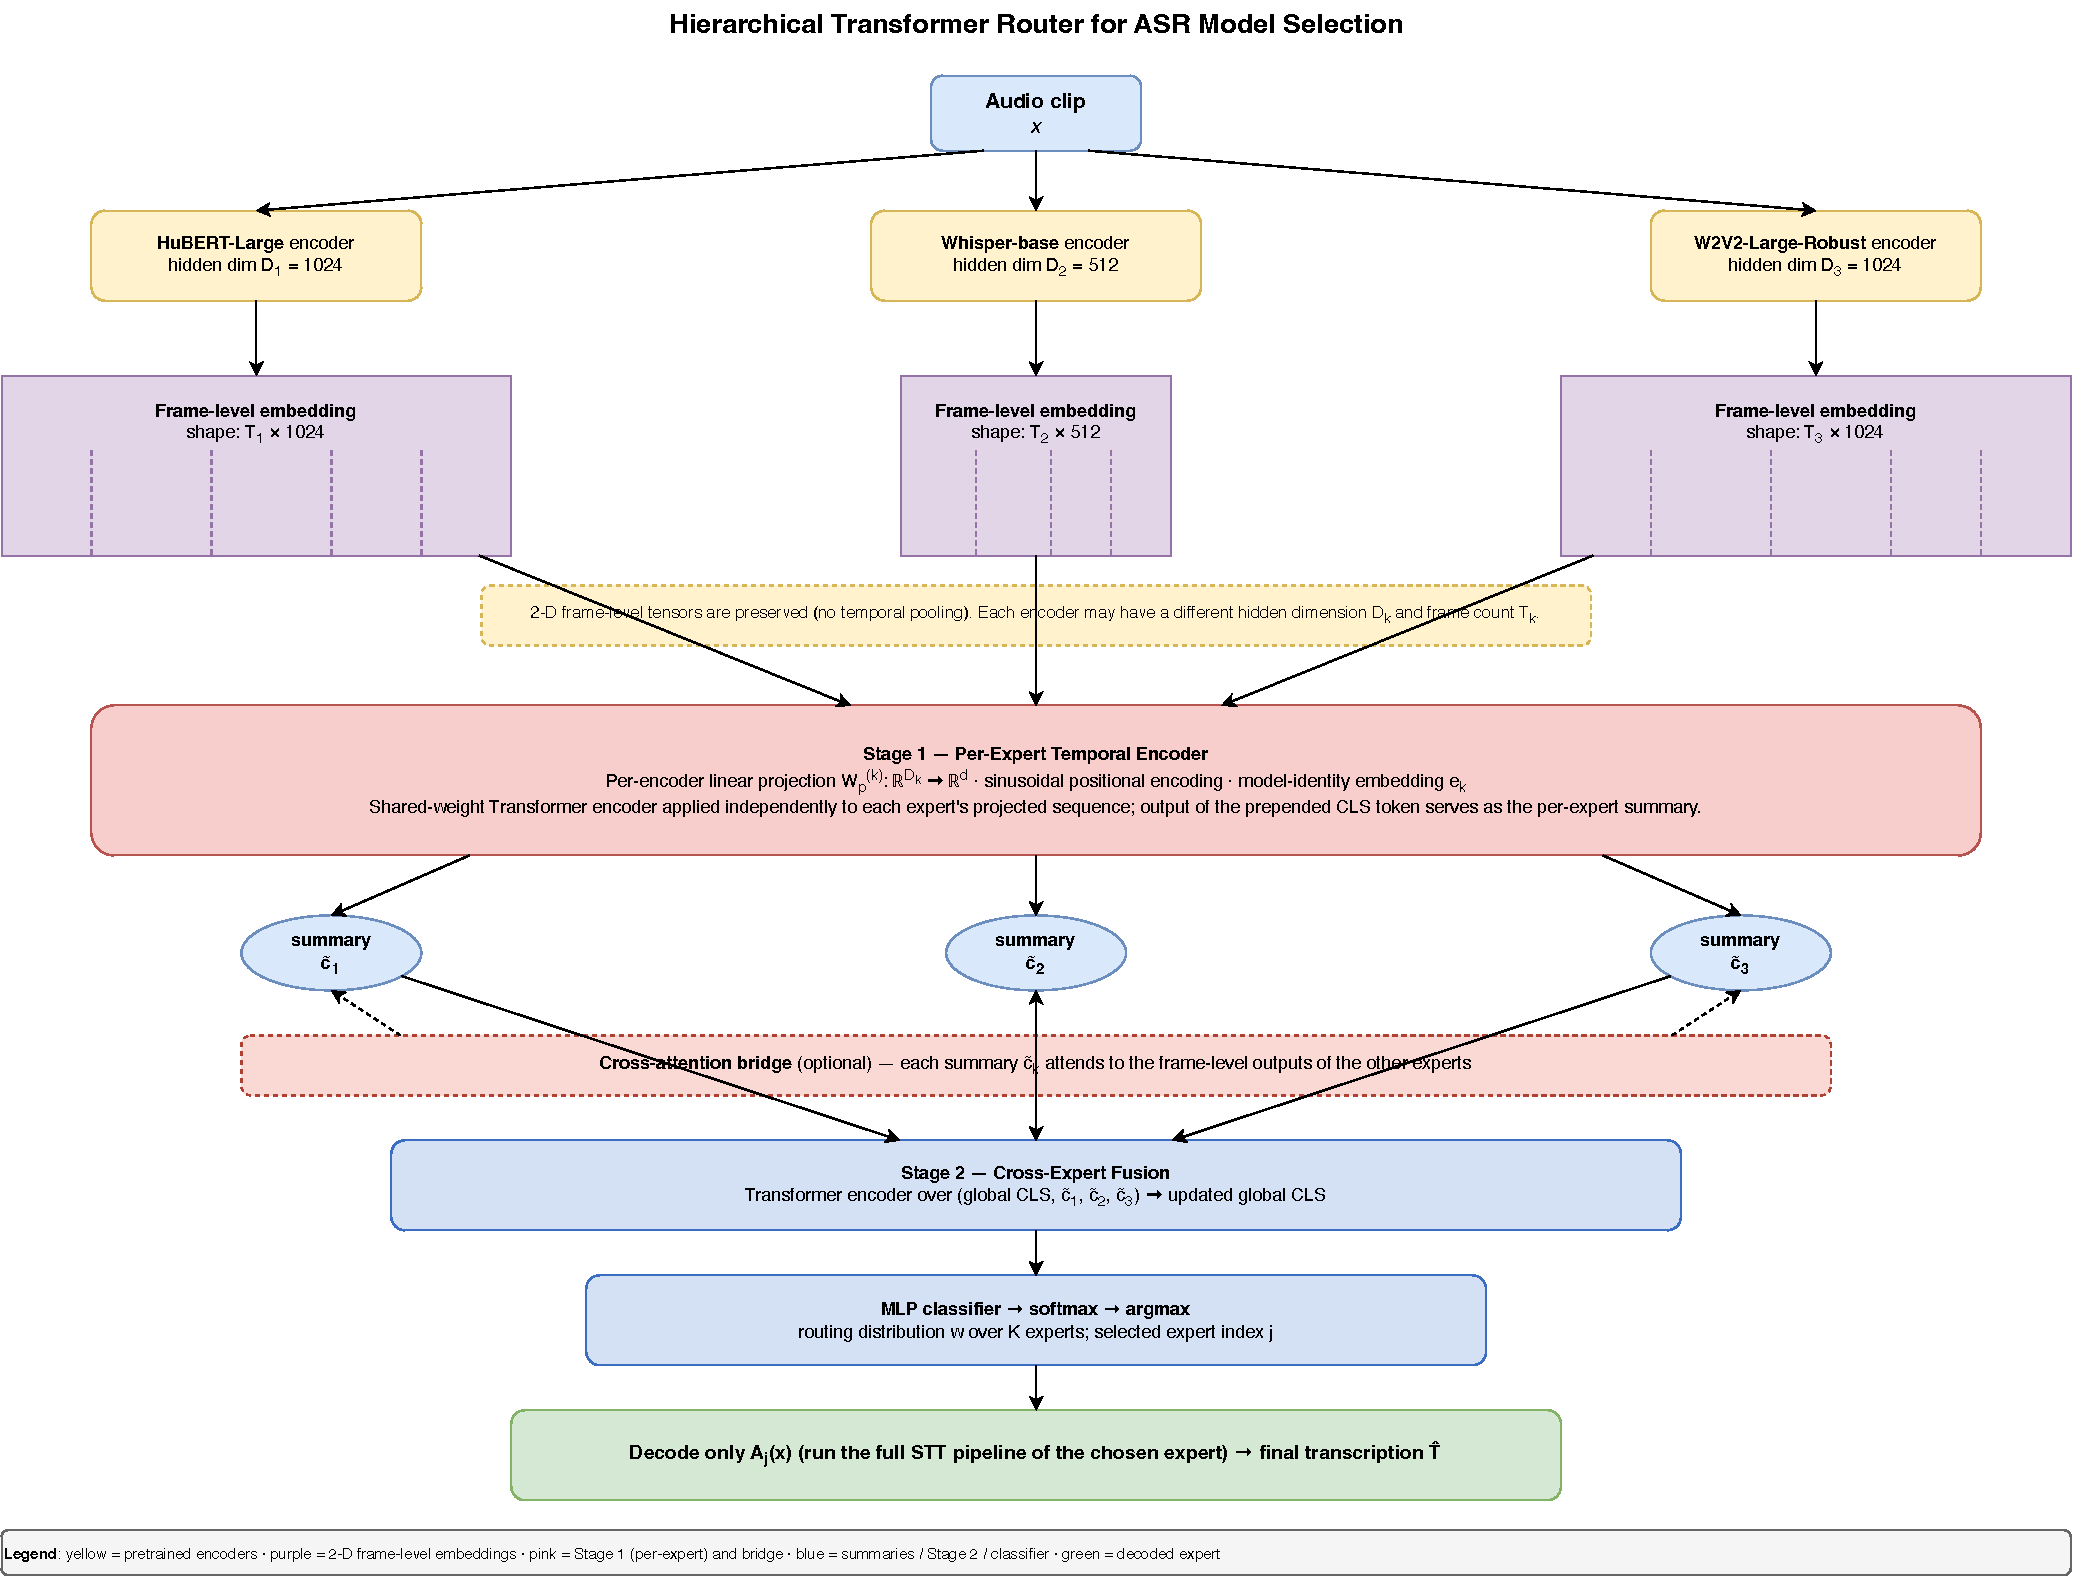
\includegraphics[width=1\linewidth]{figures/diagram.pdf}
%     \caption{Overview of the proposed sequential adaptive STT routing framework.}
%     \label{fig:sequential-routing-diagram}
% \end{figure*}

\subsection{Algorithm Overview}

The proposed framework extends adaptive STT model selection to the
sequential setting by exploiting temporal dependencies across
consecutive audio segments. The overall system operates in two
phases: an offline training phase and an online inference phase,
as illustrated in Fig.~\ref{fig:sequential-routing-diagram}. The
offline phase learns a routing model that captures how the relative
performance of different STT experts evolves across a sequence of
audio segments, while the online phase uses the trained routing model
to select an appropriate expert for each incoming segment in real time.

In the offline training phase, the system is provided with a
collection of labeled audio recordings that are partitioned into
temporally ordered segments $\{x_t\}_{t=1}^{T}$. For each segment,
a feature representation $\mathbf{z}_t$ is extracted using the
feature pipeline described in Section~\ref{sec:features}. These
representations may include acoustic descriptors, signal statistics,
and neural speech embeddings that characterize the acoustic
properties of the input segment. In contrast to independent
instance-level selection, the framework processes sequences of
segment-level representations to capture contextual relationships
across neighboring segments. For each training sequence, all STT
experts $\{A_1,\dots,A_K\}$ are evaluated on the corresponding
audio segments to obtain their transcription outputs and the
associated transcription losses defined in
Section~\ref{sec:problem}. These evaluations provide supervision
signals indicating the relative suitability of each expert for
different segments within the sequence.

Using these sequence-level observations, the routing model learns
to predict the relative performance of the candidate STT experts
conditioned on the contextual representation of the input sequence.
The parameters of the routing model are optimized during the offline
phase by minimizing the cumulative transcription loss over the
training data, allowing the system to learn how temporal patterns in
the audio stream relate to the performance of different experts.

In the online inference phase, the system receives a stream of
incoming audio segments $\{x_t\}$. For each segment, the feature
vector $\mathbf{z}_t$ is extracted as shown in
Fig.~\ref{fig:sequential-routing-diagram}. The routing model then
processes the current segment representation together with its
recent temporal context to estimate a weight vector
$\mathbf{w}_t$ over the candidate experts. A single STT algorithm
$A_{j_t}$ is selected according to the highest predicted weight,
and the final transcription $\hat{T}_t$ is obtained by executing
only the selected expert on the input segment. Because only one
STT model is executed at inference time, the proposed framework
retains the computational efficiency of single-model inference
while dynamically adapting the expert selection policy to the
evolving acoustic conditions of the audio stream.

The detailed components of the proposed framework, including the
sequence representation, the routing model, and the training
procedure, are described in the following subsections.



\textbf{Remark 1.} \textit{}

\begin{algorithm}
\small
\caption{\small Online Sequential STT Model Selection}
\label{alg:sequential-online-overview}

\textbf{Inputs:}
\begin{itemize}
    \item Incoming audio segment $x_t$
    \item Context window length $L$
    \item Set of audio feature extraction functions $\mathbb{F}(\cdot)$
    \item Trained sequential routing function $g_{\theta}(\cdot)$
    \item STT expert pool $\mathcal{A}=\{A_1,\dots,A_K\}$
\end{itemize}

\textbf{Outputs:}
\begin{itemize}
    \item Final transcription $\widehat{T}_t$ for audio segment $x_t$
\end{itemize}

\textbf{Inference Steps:}
\begin{algorithmic}[1]

\State Extract segment-level features:
\[
\mathbf{z}_t \leftarrow \mathbb{F}(x_t)
\]

\State Update contextual feature sequence:
\[
Z_t \leftarrow (\mathbf{z}_{t-L+1},\dots,\mathbf{z}_t)
\]

\State Compute expert selection scores using the routing model:
\[
\mathbf{s}_t \leftarrow g_{\theta}(Z_t)
\]

\State Normalize scores using softmax to obtain routing weights $\mathbf{w}_t$

\State Select expert model:
\[
j_t \leftarrow \arg\max_{j \in \{1,\dots,K\}} w_{t,j}
\]

\State Obtain final transcription:
\[
\widehat{T}_t \leftarrow A_{j_t}(x_t)
\]

\State Return $\widehat{T}_t$

\end{algorithmic}
\end{algorithm}




\subsection{Sequential Feature Representation}
\label{sec:features}

For each audio segment $x_t$ in the input stream, we construct a compact feature vector $\mathbf{z}_t \in \mathbb{R}^d$ that captures acoustic and contextual characteristics relevant to STT performance, as illustrated in Fig.~\ref{fig:sequential-routing-diagram}. These features summarize signal quality, phonetic content, speaker characteristics, and temporal speech dynamics \cite{rabiner1993fundamentals,li2023emotionalasr}. 

Given a sequence of audio segments $\{x_t\}_{t=1}^{T}$, the feature extraction process produces a corresponding sequence of feature vectors
\[
Z = (\mathbf{z}_1, \mathbf{z}_2, \dots, \mathbf{z}_T),
\]
which serves as a compact representation of the evolving acoustic conditions across the audio stream.

\subsubsection{Spectral–Phonetic Features}

We extract 13 Mel-frequency cepstral coefficients (MFCCs) together with their first- and second-order derivatives ($\Delta$ and $\Delta\Delta$) \cite{davis1980mfcc,furui1986deltas}. Lower-order coefficients represent the coarse spectral envelope, while higher-order terms encode finer phonetic detail. The inclusion of temporal derivatives improves robustness to coarticulation effects, speaker articulation differences, and prosodic variation \cite{rabiner1993fundamentals}. These descriptors provide a compact summary of the phonetic and spectral characteristics of each audio segment.

\subsubsection{Prosodic Features}

Prosodic features, including pitch statistics (such as mean and range) and silence ratios derived from voice activity detection (VAD), characterize speaking rhythm, stress patterns, and expressiveness \cite{boersma2001praat,sohn1999vad}. Such descriptors help identify speaking styles or acoustic conditions under which transcription accuracy may degrade, particularly in expressive or noisy speech scenarios \cite{li2023emotionalasr}.

\subsubsection{Neural Speech Embeddings}

High-level speech representations are extracted from pretrained self-supervised encoders such as Wav2Vec2 and HuBERT \cite{baevski2020wav2vec,hsu2021hubert}. These embeddings encode rich information about phonetic identity, speaker characteristics, and semantic context, complementing conventional low-level acoustic features. Since these embeddings can be obtained through a single forward pass of the pretrained encoder without performing full speech decoding, they introduce minimal computational overhead relative to running the STT models themselves.

\subsubsection{Signal and Temporal Features}

Signal-level features including signal-to-noise ratio (SNR), zero-crossing rate (ZCR), and spectral entropy quantify acoustic clarity and spectral variability \cite{schuller2013computational,eyben2015opensmile}. Temporal descriptors such as segment duration, speech rate, and pause ratio capture aspects of speaking fluency and pacing, which can significantly influence transcription robustness \cite{ko2015audio,zhang2020ttransducer}. 

\vspace{0.2cm}

The resulting feature vectors $\{\mathbf{z}_t\}_{t=1}^{T}$ collectively provide a compact sequence-level representation of the evolving acoustic conditions within the audio stream. This representation forms the basis for modeling temporal dependencies across segments and serves as the input to the routing mechanism that determines the most suitable STT expert for each segment.



\textbf{Remark 2.} \textit{}

\subsection{Transformer-Based Routing Model}
\label{subsec:transformer_router}

Given the sequence of segment-level feature vectors
\[
Z = (\mathbf{z}_1,\mathbf{z}_2,\dots,\mathbf{z}_T), \qquad \mathbf{z}_t \in \mathbb{R}^{d},
\]
obtained from the feature extraction pipeline described in
Section~\ref{sec:features}, the goal of the routing model is to
predict, for each segment $x_t$, the relative suitability of the
candidate STT experts
$\mathcal{A}=\{A_1,\dots,A_K\}$ while accounting for contextual
dependencies across neighboring segments.

To achieve this, we define a sequential routing function
\[
g_{\theta}(Z_t) = \mathbf{s}_t \in \mathbb{R}^{K},
\]
where $\theta$ denotes the trainable parameters of the routing model,
$Z_t = (\mathbf{z}_{t-L+1},\dots,\mathbf{z}_t)$ represents the contextual
feature sequence within a temporal window of length $L$, and
$\mathbf{s}_t=(s_{t,1},\dots,s_{t,K})$ denotes the routing logits
associated with the candidate experts. Each component $s_{t,j}$
represents the predicted preference score indicating how suitable
expert $A_j$ is expected to be for transcribing the current audio
segment $x_t$ given the contextual acoustic information contained in
$Z_t$.

In our framework, the routing function $g_{\theta}(\cdot)$ is
implemented using a transformer-based sequence model that maps the
input feature sequence $Z_t$ into a contextual representation. Let
\[
P_t = (\mathbf{p}_{t-L+1},\dots,\mathbf{p}_t)
\]
denote the projected feature sequence obtained by applying a linear
embedding transformation to each segment-level feature vector
\[
\mathbf{p}_i = W_e \mathbf{z}_i + b_e,
\]
where $W_e \in \mathbb{R}^{d' \times d}$ and $b_e \in \mathbb{R}^{d'}$
are learnable projection parameters. These embeddings are augmented
with positional encodings to preserve the temporal ordering of the
segments within the context window.

The embedded sequence $P_t$ is then processed by a stack of
transformer encoder layers. Each layer performs multi-head
self-attention followed by a position-wise feedforward transformation.
For an input sequence representation $H^{(\ell)}$, the attention
operation at layer $\ell$ is defined as

\[
\text{Attention}(Q,K,V) =
\text{softmax}\!\left(\frac{QK^{\top}}{\sqrt{d_k}}\right)V,
\]

where $Q$, $K$, and $V$ denote the query, key, and value matrices
derived from the input representation $H^{(\ell)}$. Through this
self-attention mechanism, the model learns contextual relationships
between neighboring segments, enabling the routing function to capture
temporal dependencies such as persistent acoustic environments,
speaker continuity, or gradual changes in signal conditions.

Let
\[
H_t = (\mathbf{h}_{t-L+1},\dots,\mathbf{h}_t)
\]
denote the contextual representations produced by the final
transformer layer. The representation corresponding to the most
recent segment, $\mathbf{h}_t$, summarizes the relevant contextual
information contained within the temporal window. This representation
is used to compute the routing logits through a linear prediction
layer

\[
\mathbf{s}_t = W_o \mathbf{h}_t + b_o,
\]

where $W_o \in \mathbb{R}^{K \times d'}$ and $b_o \in \mathbb{R}^{K}$
are learnable parameters.

To obtain normalized routing probabilities over the candidate experts,
we apply a softmax transformation to the logits:

\begin{equation}
w_{t,j} =
\frac{\exp(s_{t,j})}
{\sum_{m=1}^{K}\exp(s_{t,m})},
\qquad j=1,\dots,K,
\label{eq:sequential_router}
\end{equation}

where $w_{t,j}$ denotes the predicted probability that expert $A_j$
will produce the most accurate transcription for the current audio
segment $x_t$ given its temporal context. These probabilities quantify
the model's confidence regarding the relative suitability of the
candidate experts.

The routing decision is then obtained by selecting the expert with the
highest predicted probability, as summarized in
Algorithm~\ref{alg:sequential-online-overview}. The training procedure
for estimating the parameters $\theta$ of the routing model is
described in the following subsection.


\vspace{0.2cm}
\textbf{Remark 3.}
\textit{}

\subsection{Training Objective}
\label{subsec:training_objective}

The parameters of the sequential routing model are learned in an
offline supervised setting using labeled speech data. Let
\[
\mathcal{D}=\{(x_1,R_1),\dots,(x_T,R_T)\}
\]
denote a temporally ordered dataset of $T$ audio segments together
with their corresponding reference transcriptions. Let
$\mathcal{A}=\{A_1,\dots,A_K\}$ denote the pool of $K$ pretrained STT
experts, and let $\mathbb{F}(\cdot)$ represent the feature extraction
pipeline described in Section~\ref{sec:features}. For each audio
segment $x_t$, the feature extractor produces a segment-level feature
vector
\[
\mathbf{z}_t=\mathbb{F}(x_t).
\]

During training, all experts in $\mathcal{A}$ are evaluated on each
audio segment in order to obtain their candidate transcriptions
\[
T_{t,j}=A_j(x_t), \qquad j=1,\dots,K.
\]
These transcriptions are compared with the ground-truth reference
transcription $R_t$ to compute the corresponding transcription
errors. Using the Word Error Rate (WER) metric, the transcription
error associated with expert $A_j$ on segment $x_t$ is defined as
\[
\mathrm{WER}(T_{t,j},R_t)=\frac{S+I+D}{|R_t|},
\]
where $S$, $I$, and $D$ denote the numbers of substitutions,
insertions, and deletions obtained through a standard Levenshtein
alignment \cite{li2014overviewrobust}, and $|R_t|$ denotes the number
of words in the reference transcription.

Given the contextual feature sequence
\[
Z_t=(\mathbf{z}_{t-L+1},\dots,\mathbf{z}_t),
\]
the transformer routing model described in
Section~\ref{subsec:transformer_router} produces routing logits
\[
\mathbf{s}_t=g_{\theta}(Z_t)\in\mathbb{R}^{K}.
\]
These logits are converted into routing probabilities using the
softmax function defined in \eqref{eq:sequential_router}, producing
the expert weight vector
\[
\mathbf{w}_t=(w_{t,1},\dots,w_{t,K}),
\]
where $w_{t,j}$ represents the predicted probability that expert
$A_j$ will yield the most accurate transcription for segment $x_t$
given its contextual acoustic information.

Using these routing probabilities, we define the expected
transcription loss for segment $x_t$ as

\begin{equation}
\mathcal{L}_t =
\sum_{j=1}^{K}
w_{t,j}\,\mathrm{WER}(T_{t,j},R_t).
\label{eq:sequential_expected_loss}
\end{equation}

Intuitively, this formulation encourages the routing model to assign
higher probability mass to experts that achieve lower transcription
errors on the corresponding audio segment. By minimizing this
expected loss, the model learns to predict expert preferences that
align with the empirical performance of the STT experts.

\vspace{0.1cm}

\begin{remark}
Although WER is used as the primary optimization objective due to
its widespread adoption and interpretability in speech recognition
research \cite{yu2016asrdeep,li2014overviewrobust}, other
transcription quality metrics such as Character Error Rate (CER) or
task-specific evaluation measures could be incorporated into the
same training framework without modifying the routing architecture.
\end{remark}

The overall training objective minimizes the expected transcription
error across the entire dataset:

\begin{equation}
\min_{\theta}
\mathcal{L}
=
\frac{1}{T}
\sum_{t=1}^{T}
\mathcal{L}_t
=
\frac{1}{T}
\sum_{t=1}^{T}
\sum_{j=1}^{K}
w_{t,j}\,\mathrm{WER}(T_{t,j},R_t).
\label{eq:sequential_training_objective}
\end{equation}

During optimization, the WER values
$\mathrm{WER}(T_{t,j},R_t)$ are treated as fixed constants obtained
from offline evaluation of the STT experts. The parameters $\theta$
of the transformer routing model are then optimized using
gradient-based learning to minimize the expected transcription
loss defined in \eqref{eq:sequential_training_objective}. The
complete offline training procedure is summarized in
Algorithm~\ref{alg:sequential_offline_training}.

\begin{algorithm}
\small
\caption{Offline Training Procedure for the Sequential Routing Model}
\label{alg:sequential_offline_training}

\textbf{Inputs}
\begin{itemize}
\item $\{(x_1,R_1),\dots,(x_T,R_T)\}$: Labeled dataset of audio segments and reference transcriptions
\item $\mathbb{F}$: Feature extraction pipeline
\item $\mathcal{A}=\{A_1,\dots,A_K\}$: Pool of pretrained STT experts
\item Context window length $L$
\end{itemize}

\textbf{Output} \\
Trained routing model $g_{\theta}$

\textbf{Training Steps}

\begin{algorithmic}[1]

\State Split dataset into training and validation sets:
$\mathcal{D}_{\text{train}}, \mathcal{D}_{\text{val}}$

\For{$t \gets 1$ \textbf{to} $|\mathcal{D}_{\text{train}}|$}
    \State Extract features: $\mathbf{z}_t \gets \mathbb{F}(x_t)$
    \For{each expert $A_j \in \mathcal{A}$}
        \State Transcribe segment: $T_{t,j} \gets A_j(x_t)$
        \State Compute transcription error:
        $\mathrm{WER}_{t,j} \gets \mathrm{WER}(T_{t,j},R_t)$
    \EndFor
\EndFor

\For{each training step}
    \State Construct contextual feature sequence:
    $Z_t=(\mathbf{z}_{t-L+1},\dots,\mathbf{z}_t)$
    \State Compute routing logits:
    $\mathbf{s}_t \gets g_{\theta}(Z_t)$
    \State Compute routing probabilities using softmax
    \State Compute expected loss $\mathcal{L}_t$ using
    \eqref{eq:sequential_expected_loss}
\EndFor

\State Optimize model parameters $\theta$ using gradient-based
learning (e.g., Adam)

\State Perform early stopping and hyperparameter tuning using
validation loss on $\mathcal{D}_{\text{val}}$

\end{algorithmic}
\end{algorithm}


\textbf{Remark 4.}
\textit{}

\subsection{Temporal Consistency Regularization}

In sequential audio streams, acoustic conditions often evolve
gradually over time, and the optimal STT expert may remain stable
across consecutive segments. To encourage temporally consistent
routing decisions, we introduce a regularization term that penalizes
abrupt changes in the predicted expert distributions.

Let $\mathbf{w}_t$ and $\mathbf{w}_{t-1}$ denote the routing
probability vectors for consecutive segments. We define the temporal
consistency regularization term as
\[
\mathcal{L}_{\text{smooth}} =
\frac{1}{T-1}
\sum_{t=2}^{T}
\|\mathbf{w}_t - \mathbf{w}_{t-1}\|_2^2.
\]

The overall training objective then becomes
\begin{equation}
\min_{\theta}
\;
\mathcal{L}_{\text{total}}
=
\mathcal{L}
+
\lambda \mathcal{L}_{\text{smooth}},
\label{eq:total_objective}
\end{equation}
where $\lambda \geq 0$ controls the trade-off between transcription
accuracy and temporal stability of routing decisions.

This regularization encourages the routing model to produce smoother
expert selection trajectories, reducing unnecessary switching between
experts while still adapting to meaningful changes in acoustic
conditions.

\section{Simulations}


\section{Conclusion}
\label{sec:conclusion}

\clearpage

\bibliographystyle{ieeetr}
\bibliography{reference}





\end{document}


% %In order to address the online model selection problem defined in Section II, we propose a novel randomized switching-based meta-learning algorithm for real-time STT transcription. Unlike static ensemble methods, which aggregate predictions across all models, or deterministic selectors, which may overfit to specific conditions, our method dynamically selects a single transcription model at each time step while adaptively tracking nonstationary changes in the audio environment. The algorithm is inspired by the universal randomized switching framework and is designed to achieve sublinear regret with respect to the best piecewise-constant switching sequence in hindsight.


% \subsection*{Randomized Switching-Based Selection}

% To achieve this, we maintain a set of probability weights $\{w_{t,m}\}_{m=1}^K$ that represent the likelihood of selecting each model at time $t$. These probabilities are updated adaptively based on past losses and compactly encode all possible switching paths without requiring exponential enumeration.

% At each step $t$:
% \begin{enumerate}
%     \item \textbf{Sampling:} We sample a model index $m_n$ from a categorical distribution defined by the weight vector $\mathbf{w}_t = (w_{t,1},\ldots,w_{n,k})$:
%     \[
%     m_n \sim \mathrm{Cat}(\mathbf{w}_t), \quad \Pr[m_n = m] = w_{t,m}.
%     \]
%     The selected model produces the transcription $T_{n,m_n}$.

%     \item \textbf{Loss Observation:} The algorithm observes $\ell(T_{n,m_n}, R_n)$ for the chosen model. In a bandit setting, importance-weighted estimators can be used to obtain unbiased estimates for unobserved losses.

%     \item \textbf{Auxiliary State Update:} For each possible last-switch time $\ell \leq t$, we maintain auxiliary variables $Z_t(\ell,m)$ that accumulate exponentiated loss contributions. These variables are updated recursively according to:
%     \[
%     Z_t(\ell,m) = \beta Z_{t-1}(\ell,m) \cdot \exp(-\eta \ell(T_{n,m},R_n)) + \frac{1-\beta}{K} \sum_{j=1}^K Z_{t-1}(\ell,j),
%     \]
%     where $\eta > 0$ is a learning rate and $\beta \in (0,1)$ controls the switching penalty.

%     \item \textbf{Weight Update:} The normalized weights are then computed as
%     \[
%     w_{t+1,m} = \frac{\sum_{\ell=1}^{t} Z_t(\ell,m)}{\sum_{j=1}^K \sum_{\ell=1}^{t} Z_t(\ell,j)}.
%     \]
% \end{enumerate}

% \subsection*{Algorithmic Properties}

% The above procedure ensures that the selection strategy:
% \begin{itemize}
%     \item Tracks the best switching sequence in hindsight with expected regret bounded by $O(\sqrt{T \log T})$.
%     \item Operates with $O(K)$ update complexity per time step, making it efficient for real-time STT applications.
%     \item Naturally adapts to nonstationary environments where speaker conditions or noise profiles change abruptly or gradually.
% \end{itemize}

% \subsection*{Integration with STT Model Selection}

% In practice, each STT algorithm $M_m$ can be a large pretrained STT model (e.g., Whisper, wav2vec2, RNN-T, or domain-adapted fine-tunes). The randomized switching algorithm provides a principled way to select among them on a per-utterance basis. The stochastic nature of selection ensures continuous exploration of all candidate models, while the adaptive weight updates concentrate probability mass on those models that demonstrate superior recent performance. This framework thus provides both theoretical guarantees and practical efficiency for real-time deployment in adaptive STT systems.
